\paragraph{Hyperparameters}

\begin{figure}[t]

\hspace{-1ex}
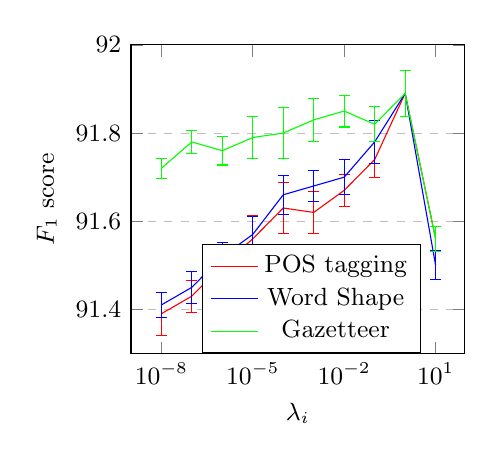
\begin{tikzpicture}
    \tikzstyle{every node}=[font=\small]

  \begin{axis}[
  	xmode=log,
  	xlabel={$\lambda_i$},
  	ylabel={$F_1$ score},
    xmin=0, xmax=90,
    ymin=91.3, ymax=92,
    height=5.5cm,
    ymajorgrids=true,
    grid style=dashed,
    width=0.48\textwidth,
%    legend pos=south east
    legend style={at={(0.87,0)},anchor=south east}
  ]

  \addplot[color=red, error bars/.cd, y dir=both, y explicit] coordinates {
  (1e-8, 91.39)+=(1e-8, 0.0484)-=(1e-8, 0.0484)
  (1e-7, 91.43)+=(1e-7, 0.0361)-=(1e-7, 0.0361)
  (1e-6, 91.50)+=(1e-6, 0.04)-=(1e-6, 0.04)
  (1e-5, 91.56)+=(1e-5, 0.0529)-=(1e-5, 0.0529)
  (1e-4, 91.63)+=(1e-4, 0.0576)-=(1e-4, 0.0576)
  (1e-3, 91.62)+=(1e-3, 0.0484)-=(1e-3, 0.0484)
  (1e-2, 91.67)+=(1e-2, 0.0361)-=(1e-2, 0.0361)
  (1e-1, 91.74)+=(1e-1, 0.04)-=(1e-1, 0.04)
  (1, 91.89)+=(1, 0.0529)-=(1, 0.0529)
  (10, 91.56)+=(10, 0.0289)-=(10, 0.0289)
  };
  \addlegendentry{POS tagging}
  
  \addplot[color=blue, error bars/.cd, y dir=both, y explicit] coordinates {
  (1e-8, 91.41)+=(1e-8, 0.0289)-=(1e-8, 0.0289)
  (1e-7, 91.45)+=(1e-7, 0.0361)-=(1e-7, 0.0361)
  (1e-6, 91.52)+=(1e-6, 0.0324)-=(1e-6, 0.0324)
  (1e-5, 91.57)+=(1e-5, 0.04)-=(1e-5, 0.04)
  (1e-4, 91.66)+=(1e-4, 0.0441)-=(1e-4, 0.0441)
  (1e-3, 91.68)+=(1e-3, 0.0361)-=(1e-3, 0.0361)
  (1e-2, 91.70)+=(1e-2, 0.04)-=(1e-2, 0.04)
  (1e-1, 91.78)+=(1e-1, 0.0484)-=(1e-1, 0.0484)
  (1, 91.89)+=(1, 0.0529)-=(1, 0.0529)
  (10, 91.50)+=(10, 0.0324)-=(10, 0.0324)
  };
  \addlegendentry{Word Shape}
  
  \addplot[color=green, error bars/.cd, y dir=both, y explicit] coordinates {
  (1e-8, 91.72)+=(1e-8, 0.0225)-=(1e-8, 0.0225)
  (1e-7, 91.78)+=(1e-7, 0.0256)-=(1e-7, 0.0256)
  (1e-6, 91.76)+=(1e-6, 0.0324)-=(1e-6, 0.0324)
  (1e-5, 91.79)+=(1e-5, 0.0484)-=(1e-5, 0.0484)
  (1e-4, 91.80)+=(1e-4, 0.0576)-=(1e-4, 0.0576)
  (1e-3, 91.83)+=(1e-3, 0.0484)-=(1e-3, 0.0484)
  (1e-2, 91.85)+=(1e-2, 0.0361)-=(1e-2, 0.0361)
  (1e-1, 91.82)+=(1e-1, 0.04)-=(1e-1, 0.04)
  (1, 91.89)+=(1, 0.0529)-=(1, 0.0529)
  (10, 91.56)+=(10, 0.0289)-=(10, 0.0289)
  };
  \addlegendentry{Gazetteer}
  \end{axis}
\end{tikzpicture}
%}

\vspace{-2ex}
\caption{Effect of hyperparameter values on model performance. Each curve shows the effect of $\lambda_i$, for feature type $i$, with all other $\lambda_j=1, ~j \ne i$. Performance averaged over 5 runs, and error bars show $\pm$ 1 variance.}
\label{figure3}
\end{figure}

Three extra hyperparameters are introduced into our model, controlling the weight of the autoencoder loss relative to the CRF loss, for each feature type.
\figref{figure3} shows the effect of each hyperparameter on test performance. 
Observe that setting $\lambda_i=1$ gives strong performance, and that the impact of the gazetteer is less marked than the other two feature types. 
While increasing $\lambda$ is mostly beneficial, performance drops if the $\lambda s$ are overly large, that is, the auto-encoder loss overwhelms the main prediction task.
